\documentclass[tikz,border=15pt]{standalone}
\usepackage{tikz}
\usetikzlibrary{positioning, arrows.meta, calc}

\begin{document}

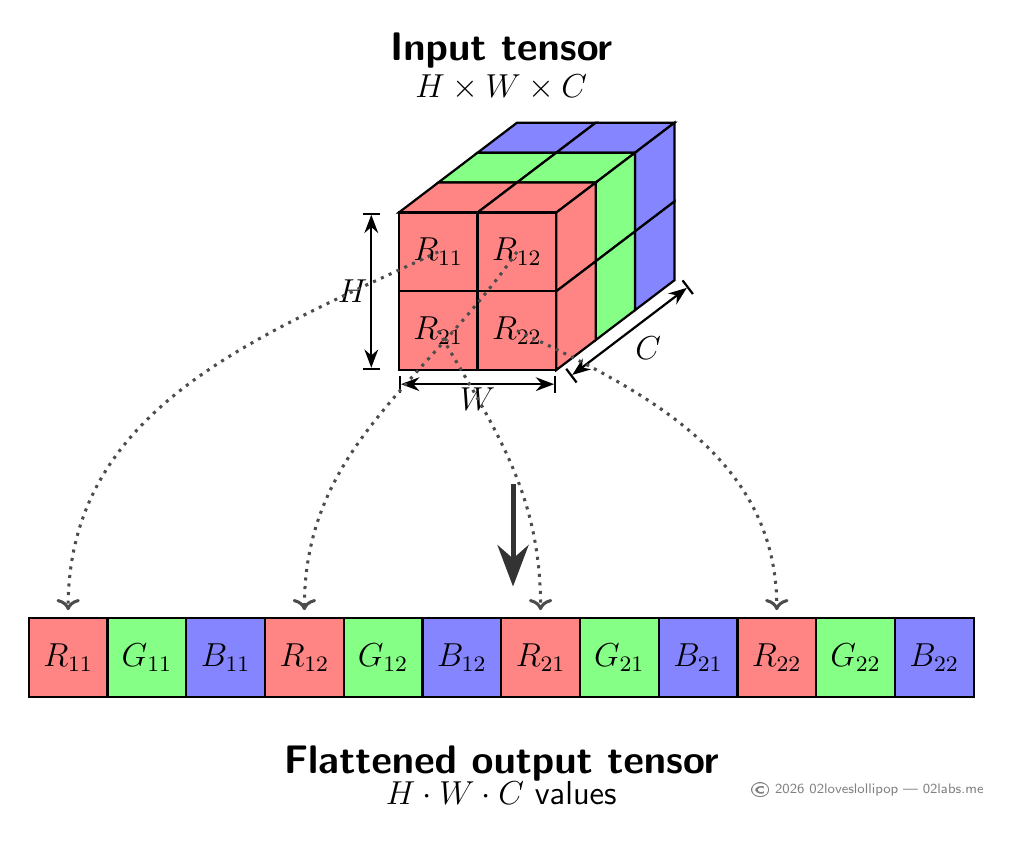
\begin{tikzpicture}[
    x={(1cm,0cm)},
    y={(0cm,1cm)},
    z={(0.5cm,0.38cm)},
    font=\sffamily\large
]

\colorlet{colR}{red!48}
\colorlet{colG}{green!48}
\colorlet{colB}{blue!48}

% 3D input tensor: draw back-to-front so the visible faces overlap cleanly.
\foreach \z/\col/\chan in {2/colB/B, 1/colG/G, 0/colR/R} {
    \foreach \y [count=\yi] in {1, 0} {
        \foreach \x [count=\xi] in {0, 1} {
            \ifnum\y=1
                \draw[fill=\col, draw=black, thick]
                    (\x, \y+1, \z) -- (\x+1, \y+1, \z) --
                    (\x+1, \y+1, \z+1) -- (\x, \y+1, \z+1) -- cycle;
            \fi

            \ifnum\x=1
                \draw[fill=\col, draw=black, thick]
                    (\x+1, \y, \z) -- (\x+1, \y+1, \z) --
                    (\x+1, \y+1, \z+1) -- (\x+1, \y, \z+1) -- cycle;
            \fi

            \ifnum\z=0
                \draw[fill=\col, draw=black, thick]
                    (\x, \y, \z) -- (\x+1, \y, \z) --
                    (\x+1, \y+1, \z) -- (\x, \y+1, \z) -- cycle;
                \node at (\x+0.5, \y+0.5, \z) {$\chan_{\yi\xi}$};
            \fi
        }
    }
}

\draw[|<->|, >=Stealth, thick] (-0.35, 0, 0) -- (-0.35, 2, 0) node[midway, left, fill=white, inner sep=1pt] {$H$};
\draw[|<->|, >=Stealth, thick] (0, -0.18, 0) -- (2, -0.18, 0) node[midway, below, fill=white, inner sep=1pt] {$W$};
\draw[|<->|, >=Stealth, thick] (2.18, -0.08, 0) -- (2.18, -0.08, 3) node[midway, below right=1pt, fill=white, inner sep=1pt] {$C$};

\node[anchor=south, font=\sffamily\Large\bfseries, fill=white, inner sep=2pt] at (1.3, 3.75, 0) {Input tensor};
\node[anchor=south, font=\sffamily\large, fill=white, inner sep=2pt] at (1.3, 3.35, 0) {$H \times W \times C$};

% 1D flattened tensor: row, then column, then RGB channel.
\begin{scope}[shift={(-4.7, -4.15, 0)}]
    \foreach \yi [count=\y] in {1, 2} {
        \foreach \xi [count=\x] in {1, 2} {
            \foreach \z/\col/\chan [count=\c] in {0/colR/R, 1/colG/G, 2/colB/B} {
                \pgfmathtruncatemacro{\idx}{(\y-1)*6 + (\x-1)*3 + (\c-1)}
                \draw[fill=\col, draw=black, thick] (\idx, 0) rectangle (\idx+1, 1);
                \node at (\idx+0.5, 0.5) {$\chan_{\yi\xi}$};
            }
        }
    }

    \node[anchor=north, font=\sffamily\Large\bfseries] at (6, -0.5, 0) {Flattened output tensor};
\node[anchor=north, font=\sffamily\large] at (6, -0.95, 0) {$H \cdot W \cdot C$ values};
\end{scope}

\draw[-{Stealth[scale=1.35]}, line width=1.8pt, draw=black!80]
    (1.45, -1.45, 0) to[out=-90, in=90] (1.45, -2.75, 0);

\draw[->, dotted, line width=1.1pt, black!70]
    (0.5, 1.5, 0) to[out=205, in=90] (-4.2, -3.05, 0);
\draw[->, dotted, line width=1.1pt, black!70]
    (1.5, 1.5, 0) to[out=235, in=90] (-1.2, -3.05, 0);
\draw[->, dotted, line width=1.1pt, black!70]
    (0.5, 0.5, 0) to[out=300, in=90] (1.8, -3.05, 0);
\draw[->, dotted, line width=1.1pt, black!70]
    (1.5, 0.5, 0) to[out=335, in=90] (4.8, -3.05, 0);

% Redraw important labels last so the guide lines never cut through text.
\node[anchor=south, font=\sffamily\Large\bfseries, fill=white, inner sep=2pt] at (1.3, 3.75, 0) {Input tensor};
\node[anchor=south, font=\sffamily\large, fill=white, inner sep=2pt] at (1.3, 3.35, 0) {$H \times W \times C$};

\node[anchor=south east, font=\sffamily\tiny, text=gray] at (7.55, -5.55, 0)
    {\copyright\ 2026 02loveslollipop | 02labs.me};

\end{tikzpicture}

\end{document}
